\documentclass[11pt]{article}
\usepackage[margin=0.8in]{geometry}
\usepackage{booktabs}
\usepackage{graphicx}
\usepackage{microtype}
\usepackage[round,authoryear]{natbib}
\usepackage{xcolor}
\usepackage[colorlinks=true,allcolors=blue!55!black]{hyperref}
\graphicspath{{generated/}}
% Generated from aggregate ANTs outputs; do not edit by hand.
\newcommand{\AntsManifestN}{214}
\newcommand{\AntsRegistrationPassN}{214}
\newcommand{\AntsDeformationPassN}{213}
\newcommand{\AntsAnalysisN}{210}
\newcommand{\AntsHodgePassN}{214}
\newcommand{\AntsBrainDiceMedian}{0.971}
\newcommand{\AntsCycleMedian}{0.075}
\newcommand{\AntsCycleMaximum}{0.094}
\newcommand{\AntsRawFoldingMaximum}{0.000\%}
\newcommand{\AntsDeformationAdvantage}{0.81}
\newcommand{\AntsDeformationCILow}{0.004}
\newcommand{\AntsDeformationCIHigh}{1.608}
\newcommand{\AntsDeformationP}{0.038}
\newcommand{\AntsHodgeAdvantage}{-0.12}
\newcommand{\AntsHodgeCILow}{-0.53}
\newcommand{\AntsHodgeCIHigh}{0.30}
\newcommand{\AntsHodgeP}{0.507}
\newcommand{\AntsAdjustedMagnitudeRho}{-0.145}
\newcommand{\AntsAdjustedMagnitudeP}{0.182}
\newcommand{\AntsAdjustedCurlFreeRho}{-0.131}
\newcommand{\AntsAdjustedCurlFreeP}{0.182}
\newcommand{\AntsAdjustedDivergenceFreeRho}{0.141}
\newcommand{\AntsAdjustedDivergenceFreeP}{0.182}
\newcommand{\AntsMagnitudeAgreement}{0.178}
\newcommand{\AntsTotalRMSAgreement}{0.130}
\newcommand{\AntsCurlFreeAgreement}{0.257}
\newcommand{\AntsDivergenceFreeAgreement}{0.259}
\newcommand{\AntsVsSvregDeformationDifference}{-0.44}
\newcommand{\AntsVsSvregDeformationCILow}{-1.20}
\newcommand{\AntsVsSvregDeformationCIHigh}{0.27}
\newcommand{\AntsVsSvregHodgeDifference}{0.06}
\newcommand{\AntsVsSvregHodgeCILow}{-0.41}
\newcommand{\AntsVsSvregHodgeCIHigh}{0.55}
\newcommand{\AntsVsSvregCombinedDifference}{-0.34}
\newcommand{\AntsVsSvregCombinedCILow}{-1.02}
\newcommand{\AntsVsSvregCombinedCIHigh}{0.32}


\title{Supplementary Material 2: Independent ANTs/MNI152 Registration-Pipeline Analysis in
Symmetric MNI152 Space}
\author{Anand A. Joshi}
\date{}

\renewcommand{\thetable}{A\arabic{table}}
\renewcommand{\thefigure}{A\arabic{figure}}

\begin{document}
\maketitle

\section{Purpose and scope}

This analysis tests whether the study's geometric and behavioral conclusions
depend on the atlas-registration pipeline. It repeats deformation
extraction, stationary-log/Helmholtz--Hodge analysis, descriptive and adjusted
associations, and leakage-resistant nested cross-validation after independently
registering the same lesion-filled anatomical images with ANTs. The input
anatomy, lesion masks, inpainting targets, clinical table, outcomes, feature
definitions, and statistical plan were held constant; registration software,
reference atlas, and working resolution changed together. This is therefore a
whole-pipeline sensitivity analysis, not an isolated ANTs-versus-SVReg software
experiment. Agreement does not establish physical validity; disagreement
identifies pipeline dependence.

\section{ANTs registration to and from MNI152}

The fixed reference was the 1-mm symmetric ICBM 152 nonlinear 2009a template
(MNI152NLin2009aSym) and brain mask retrieved programmatically from TemplateFlow
\citep{Fonov2009,Ciric2022}. Code verified canonical RAS orientation,
orthogonal axes, an odd first dimension, a central voxel at world $x=0$, and
exact reflection symmetry of the brain mask. These checks are necessary because
an array reversal is not a valid contralateral reflection in every nominal MNI
geometry.

Each lesion-filled, brain-extracted T1-weighted image was resampled to 2-mm
isotropic resolution and registered to the fixed reference with ANTsPy 0.6.1
using rigid, affine, and symmetric normalization (SyN) stages
\citep{Avants2008,Avants2011}. Fixed and moving brain masks constrained all
stages. The reproducible quick preset
\texttt{antsRegistrationSyNQuickRepro[s]} used cross-correlation for the SyN
stage, random seed 2026, single-precision arithmetic, and one ITK thread per
case. Process-level parallelism did not change within-case threading or seed.
The single SyN fit supplied forward and inverse mappings. Subject-to-MNI image
resampling and MNI-to-subject image resampling were both saved outside the
repository, together with the affine, forward warp, and inverse warp.

The quick reproducible schedule was selected after an engineering benchmark on
one case. Relative to the full reproducible schedule, elapsed time decreased
from 348.3 to 87.8 seconds, brain-mask Dice changed from 0.9012 to 0.9008, and
intensity correlation changed from 0.5643 to 0.5493. This computational
benchmark motivated a feasible complete-cohort rerun and is not cohort-level
biological evidence.

ANTs applies transformations to images by pull resampling, whereas its point
interface uses the forward list to map fixed points to moving points. We
therefore transformed every fixed-brain voxel center through the forward list
to construct the fixed-to-moving inverse coordinate map required by the main
analysis. A deterministic sample of approximately 2,000 points was then mapped
back with the inverse list. Registration QC required fixed--warped-moving brain
Dice $\geq0.70$, round-trip RMSE $\leq0.50$ mm, and a nonpositive-Jacobian
fraction $\leq0.001$ in the raw SyN warp.

\section{Deformation and log-domain analysis}

The fixed-to-moving coordinate map was analyzed with the same
contralesional-affine removal, mirrored homolog subtraction, exclusion masks,
2-mm physical smoothing, 3--20-mm shell, and laterality criterion as the main
analysis. The 1,000-voxel support criterion of the 1-mm analysis was expressed
as its resolution-invariant physical equivalent of 1,000 mm$^3$, or 125 voxels
on the 2-mm grid. Affine-fit residuals were converted from 2-mm source voxels
to millimetres before reporting.

Stationary-log and Helmholtz--Hodge settings preserved the physical construction
of the main analysis: a 2-voxel stride produced a 4-mm analysis grid; taper,
smoothing, padding, exponentiation, and reconstruction criteria were unchanged.
The representation remains an arbitrary-unit stationary registration parameter,
not measured tissue velocity. No pressure, force, or tissue-mechanics parameter
was estimated.

The same clinical and conventional lesion predictors, uncertainty features,
ridge-penalty grid, 20 repeated nested five-fold splits, bootstrap sample count,
association families, multiplicity corrections, and left-lesion-only analysis
were regenerated. Because the retained participants and deterministic ordering
matched the SVReg analysis, the common predictive models used identical outer
splits. ANTs--SVReg descriptor agreement used Spearman correlation with
participant-bootstrap 95\% intervals. Direct algorithmic prediction comparisons
used participant mean absolute error averaged over repeats; positive
ANTs-minus-SVReg values favor SVReg.

ANTs registration did not include the direct non-inpainted SVReg rerun. The two
descriptive correlations involving that SVReg-only sensitivity quantity were
therefore omitted rather than represented by artificial zeros; Holm correction
covered the ten measured ANTs descriptive associations. The six adjusted
associations were unchanged in definition.

\section{Registration and field quality control}

The ANTs manifest contained \AntsManifestN{} cases.
\AntsRegistrationPassN{} passed registration QC and \AntsDeformationPassN{}
passed the combined registration/deformation criteria. Median brain-mask Dice
was \AntsBrainDiceMedian{}. Median round-trip RMSE was \AntsCycleMedian{} mm
(maximum \AntsCycleMaximum{} mm), and the maximum raw-warp nonpositive-Jacobian
fraction was \AntsRawFoldingMaximum{}. All \AntsHodgePassN{} extracted
stationary-log embeddings passed log-domain QC. Complete distributions are in
Table~\ref{tab:ants-qc} and Figure~\ref{fig:ants-qc}.

\begin{table}[ht]
\centering
\caption{Complete ANTs registration and deformation quality-control summaries.}
\label{tab:ants-qc}
\scriptsize
\resizebox{\textwidth}{!}{\begin{tabular}{lrrrrr}
\toprule
Metric & Min & Q1 & Median & Q3 & Max \\
\midrule
Brain-mask Dice & 0.8668 & 0.9631 & 0.9715 & 0.9764 & 0.9830 \\
Cycle RMSE (mm) & 0.0502 & 0.0701 & 0.0749 & 0.0795 & 0.0939 \\
Cycle maximum (mm) & 0.2925 & 0.4147 & 0.4831 & 0.5538 & 0.8659 \\
Intensity Pearson r & 0.4720 & 0.6547 & 0.6995 & 0.7236 & 0.7791 \\
Raw minimum Jacobian & 0.1158 & 0.2719 & 0.3111 & 0.3467 & 0.4450 \\
Raw folding fraction & 0.0000 & 0.0000 & 0.0000 & 0.0000 & 0.0000 \\
Normalized-field folding fraction & 0.0017 & 0.0062 & 0.0077 & 0.0096 & 0.0218 \\
Affine-fit RMSE (mm) & 2.2053 & 2.8571 & 3.0364 & 3.2995 & 4.5001 \\
\bottomrule
\end{tabular}
}
\end{table}

\begin{figure}[ht]
\centering
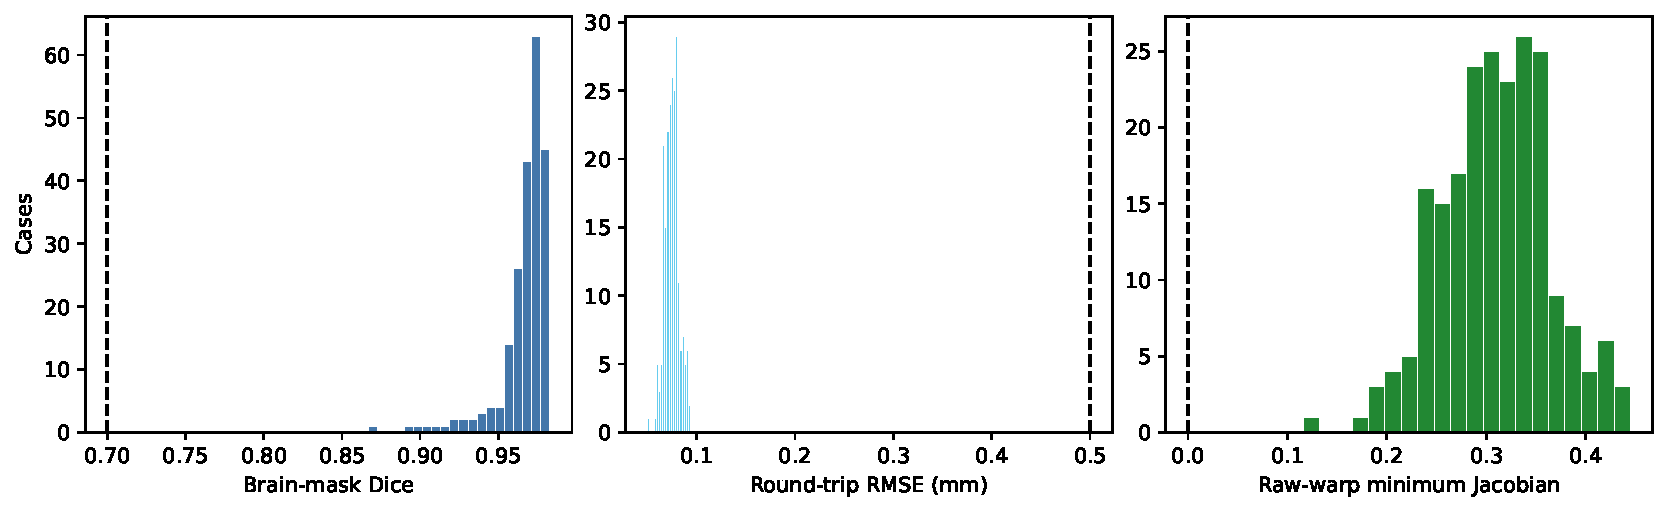
\includegraphics[width=\textwidth]{registration_qc.pdf}
\caption{\textbf{ANTs registration quality control.} Dashed lines show the
predefined eligibility boundaries. The Jacobian boundary is zero.}
\label{fig:ants-qc}
\end{figure}

\section{Cross-algorithm descriptor agreement}

Spearman rank agreement between ANTs and SVReg was
$\rho=\AntsMagnitudeAgreement$ for median near-lesion displacement magnitude,
$\rho=\AntsTotalRMSAgreement$ for stationary-log RMS,
$\rho=\AntsCurlFreeAgreement$ for curl-free energy fraction, and
$\rho=\AntsDivergenceFreeAgreement$ for divergence-free energy fraction.
Table~\ref{tab:ants-agreement} reports all displacement and Hodge descriptors,
including bootstrap intervals. Rank agreement quantifies pipeline sensitivity;
it is not an equivalence test.

\begin{table}[ht]
\centering
\caption{ANTs--SVReg descriptor rank agreement on common QC-passing cases.}
\label{tab:ants-agreement}
\scriptsize
\resizebox{\textwidth}{!}{\begin{tabular}{lrrrrr}
\toprule
Family & Descriptor & n & $\rho$ & CI low & CI high \\
\midrule
Displacement & Median magnitude & 213 & 0.178 & 0.040 & 0.308 \\
Displacement & 95th-percentile magnitude & 213 & 0.358 & 0.228 & 0.479 \\
Displacement & Median signed radial & 213 & 0.664 & 0.571 & 0.744 \\
Displacement & Mean absolute radial & 213 & 0.287 & 0.155 & 0.413 \\
Displacement & Outward radial integral & 213 & 0.769 & 0.699 & 0.825 \\
Displacement & Inward radial integral & 213 & 0.677 & 0.590 & 0.748 \\
Displacement & Log-Jacobian expansion integral & 213 & 0.689 & 0.598 & 0.763 \\
Displacement & Log-Jacobian compression integral & 213 & 0.842 & 0.786 & 0.884 \\
Hodge & Log-velocity RMS & 214 & 0.130 & -0.008 & 0.256 \\
Hodge & Curl-free energy fraction & 214 & 0.257 & 0.124 & 0.376 \\
Hodge & Divergence-free energy fraction & 214 & 0.259 & 0.129 & 0.388 \\
\bottomrule
\end{tabular}
}
\end{table}

\begin{figure}[ht]
\centering
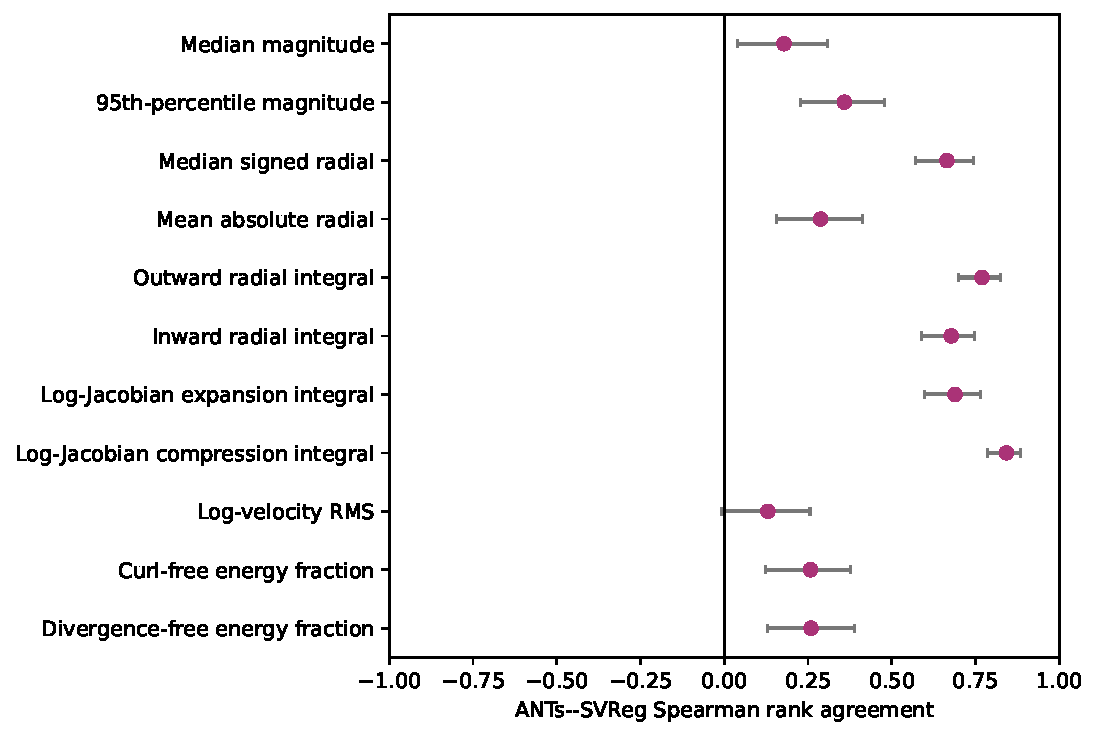
\includegraphics[width=0.9\textwidth]{descriptor_agreement.pdf}
\caption{\textbf{ANTs--SVReg rank agreement.} Points are Spearman
correlations; bars are participant-bootstrap 95\% intervals.}
\label{fig:ants-agreement}
\end{figure}

\section{Complete ANTs associations, including nonsignificant results}

Table~\ref{tab:ants-associations} reports the complete prespecified unadjusted
association family. Table~\ref{tab:ants-adjusted} reports all adjusted
associations after rank residualization on the conventional clinical and lesion
variables. The adjusted magnitude association was partial
$\rho=\AntsAdjustedMagnitudeRho$ (Holm $p=\AntsAdjustedMagnitudeP$), the
curl-free association was $\rho=\AntsAdjustedCurlFreeRho$ (Holm
$p=\AntsAdjustedCurlFreeP$), and the divergence-free association was
$\rho=\AntsAdjustedDivergenceFreeRho$ (Holm
$p=\AntsAdjustedDivergenceFreeP$).

\begin{table}[ht]
\centering
\caption{Complete ANTs descriptive Spearman association family.}
\label{tab:ants-associations}
\scriptsize
\resizebox{\textwidth}{!}{\begin{tabular}{lrrrrr}
\toprule
Association & n & $\rho$ & CI low & CI high & Holm p \\
\midrule
Lesion volume vs AQ & 210 & -0.698 & -0.769 & -0.612 & $<$0.001 \\
Magnitude vs lesion volume & 210 & 0.139 & -0.004 & 0.274 & 0.045 \\
Absolute radial vs lesion volume & 210 & 0.291 & 0.157 & 0.416 & $<$0.001 \\
Magnitude vs AQ & 210 & -0.184 & -0.316 & -0.048 & 0.022 \\
Absolute radial vs AQ & 210 & -0.270 & -0.394 & -0.134 & $<$0.001 \\
Signed radial vs AQ & 210 & -0.277 & -0.395 & -0.149 & $<$0.001 \\
Log-velocity RMS vs lesion volume & 210 & -0.462 & -0.567 & -0.345 & $<$0.001 \\
Log-velocity RMS vs AQ & 210 & 0.377 & 0.255 & 0.483 & $<$0.001 \\
Curl-free fraction vs AQ & 210 & -0.212 & -0.340 & -0.078 & 0.008 \\
Divergence-free fraction vs AQ & 210 & 0.168 & 0.033 & 0.294 & 0.030 \\
\bottomrule
\end{tabular}
}
\end{table}

\begin{table}[ht]
\centering
\caption{Complete ANTs conventional-feature-adjusted association family.}
\label{tab:ants-adjusted}
\scriptsize
\resizebox{\textwidth}{!}{\begin{tabular}{lrrrrr}
\toprule
Association & n & Partial $\rho$ & CI low & CI high & Holm p \\
\midrule
Magnitude vs AQ & 210 & -0.145 & -0.271 & -0.012 & 0.182 \\
Absolute radial vs AQ & 210 & -0.118 & -0.248 & 0.020 & 0.182 \\
Signed radial vs AQ & 210 & -0.152 & -0.282 & -0.016 & 0.149 \\
Log-velocity RMS vs AQ & 210 & 0.069 & -0.064 & 0.207 & 0.315 \\
Curl-free fraction vs AQ & 210 & -0.131 & -0.272 & 0.023 & 0.182 \\
Divergence-free fraction vs AQ & 210 & 0.141 & -0.010 & 0.280 & 0.182 \\
\bottomrule
\end{tabular}
}
\end{table}

\section{Complete predictive results and direct algorithm comparison}

The ANTs analysis cohort contained \AntsAnalysisN{} participants. Adding ANTs
deformation features to the conventional lesion model produced a mean MAE
advantage of \AntsDeformationAdvantage{} points (95\% interval
\AntsDeformationCILow{} to \AntsDeformationCIHigh{}; Holm
$p=\AntsDeformationP$). Adding ANTs Hodge features produced an advantage of
\AntsHodgeAdvantage{} points (\AntsHodgeCILow{} to \AntsHodgeCIHigh{}; Holm
$p=\AntsHodgeP$). Tables~\ref{tab:ants-models} and
\ref{tab:ants-paired} retain every evaluated model and comparison, including
nonsignificant findings.

\begin{table}[ht]
\centering
\caption{Complete repeated nested-CV results using ANTs-derived features.}
\label{tab:ants-models}
\scriptsize
\resizebox{\textwidth}{!}{\begin{tabular}{lrrrrr}
\toprule
Model & n & MAE & RMSE & $R^2$ & $r$ \\
\midrule
Intercept only & 210 & 24.14 & 27.68 & -0.009 & -0.119 \\
Clinical & 210 & 24.23 & 27.83 & -0.020 & -0.132 \\
Conventional lesion & 210 & 16.42 & 20.36 & 0.454 & 0.675 \\
Lesion + deformation & 210 & 15.61 & 19.55 & 0.497 & 0.705 \\
Lesion + uncertainty & 210 & 15.71 & 20.11 & 0.468 & 0.688 \\
Uncertainty + deformation & 210 & 15.29 & 19.28 & 0.510 & 0.715 \\
Lesion + log-velocity Hodge & 210 & 16.54 & 20.45 & 0.449 & 0.672 \\
Deformation + log-velocity Hodge & 210 & 15.78 & 19.65 & 0.492 & 0.702 \\
\bottomrule
\end{tabular}
}
\end{table}

\begin{table}[ht]
\centering
\caption{Complete paired MAE comparisons using ANTs-derived features.}
\label{tab:ants-paired}
\scriptsize
\resizebox{\textwidth}{!}{\begin{tabular}{lrrrrr}
\toprule
Reference & Comparison & Advantage & CI low & CI high & Holm p \\
\midrule
Conventional lesion & Clinical & -7.81 & -9.88 & -5.71 & $<$0.001 \\
Conventional lesion & Lesion + deformation & 0.81 & 0.004 & 1.61 & 0.038 \\
Conventional lesion & Lesion + uncertainty & 0.71 & -0.09 & 1.50 & 0.008 \\
Conventional lesion & Uncertainty + deformation & 1.13 & 0.35 & 1.91 & 0.005 \\
Conventional lesion & Intercept only & -7.72 & -9.73 & -5.64 & $<$0.001 \\
Conventional lesion & Lesion + log-velocity Hodge & -0.12 & -0.53 & 0.30 & 0.507 \\
Conventional lesion & Deformation + log-velocity Hodge & 0.64 & -0.18 & 1.47 & 0.114 \\
Lesion + uncertainty & Uncertainty + deformation & 0.42 & -0.24 & 1.10 & 0.162 \\
Lesion + deformation & Deformation + log-velocity Hodge & -0.17 & -0.47 & 0.11 & 0.292 \\
\bottomrule
\end{tabular}
}
\end{table}

On identical participants and splits, ANTs-minus-SVReg mean MAE was
\AntsVsSvregDeformationDifference{} points for the deformation-augmented model
(95\% interval \AntsVsSvregDeformationCILow{} to
\AntsVsSvregDeformationCIHigh{}), \AntsVsSvregHodgeDifference{} for the
Hodge-augmented model (\AntsVsSvregHodgeCILow{} to
\AntsVsSvregHodgeCIHigh{}), and \AntsVsSvregCombinedDifference{} for the
combined model (\AntsVsSvregCombinedCILow{} to
\AntsVsSvregCombinedCIHigh{}). Table~\ref{tab:ants-predictive-method}
reports all common models; the shared conventional model is included as a
zero-difference implementation check.

\begin{table}[ht]
\centering
\caption{Direct ANTs--SVReg prediction comparison on shared outer-CV splits.
Positive $\Delta$MAE indicates larger error with ANTs.}
\label{tab:ants-predictive-method}
\scriptsize
\resizebox{\textwidth}{!}{\begin{tabular}{lrrrrrr}
\toprule
Model & SVReg MAE & ANTs MAE & $\Delta$MAE & CI low & CI high & p \\
\midrule
Clinical & 24.23 & 24.23 & 0.00 & 0.00 & 0.00 & 1.000 \\
Intercept only & 24.14 & 24.14 & 0.00 & 0.00 & 0.00 & 1.000 \\
Lesion + log-velocity Hodge & 16.48 & 16.54 & 0.06 & -0.41 & 0.55 & 0.590 \\
Lesion + deformation & 16.04 & 15.61 & -0.44 & -1.20 & 0.27 & 0.681 \\
Deformation + log-velocity Hodge & 16.12 & 15.78 & -0.34 & -1.02 & 0.32 & 0.628 \\
Lesion + uncertainty & 15.71 & 15.71 & 0.00 & 0.00 & 0.00 & 1.000 \\
Conventional lesion & 16.42 & 16.42 & 0.00 & 0.00 & 0.00 & 1.000 \\
Uncertainty + deformation & 15.77 & 15.29 & -0.48 & -1.07 & 0.05 & 0.228 \\
\bottomrule
\end{tabular}
}
\end{table}

\section{Interpretation and limitations}

This sensitivity analysis changes the nonlinear registration implementation,
reference atlas, and working resolution, but not lesion delineation,
inpainting, behavioral measurements, or conventional lesion predictors. It
therefore addresses whole-pipeline dependence, not an isolated software effect
or all sources of measurement uncertainty. Agreement may remain inflated by
shared input preprocessing, while disagreement can arise from reference
anatomy, optimizer, similarity metric, regularization, or resolution. The
2-mm registration grid and reproducible quick schedule prioritize a feasible,
fully regenerated cohort analysis; they do not reproduce the precise scale of
SVReg optimization. Finally, neither a diffeomorphic ANTs warp nor a stable
Hodge component supplies the constitutive parameters and boundary conditions
required for pressure inference.

The within-ANTs deformation comparison met its prespecified criterion, but its
lower bootstrap bound was close to zero, the corresponding SVReg comparison
was inconclusive, and the direct same-split ANTs--SVReg MAE interval included
zero. The appropriate interpretation is pipeline-sensitive evidence rather
than a replicated deformation biomarker or a demonstrated advantage of one
registration package.

\bibliographystyle{apalike}
\bibliography{../../paper/references}

\end{document}
